\documentclass{article}
\usepackage{cleveref}
\usepackage{booktabs}
\usepackage{graphicx}
\usepackage{float}
\restylefloat{table}

\author{Alex Seewald}
\title{Wikipedia Usage Analytics}
\begin{document}

\maketitle

The software infrastructure of my big data project takes as an instance a \texttt{(referer int, page\_id int, pairwise\_views int, referer\_name varchar, page\_name varchar, type varchar)} relation and set of labeled (either experimental group or control group) categories, each of which has a set of titles which are represented as a \texttt{page\_name} in the relation. The user does not manually specify random selection as a control group category; that is done automatically. From such an instance, a solution is computed (on the $10^1$ second timescale) which contains the table in \cref{tab:struct}, along with useful reductions of that table. Although the 3.1 GB tab-seperated-value file released by wikipedia fits the shape of my problem, I manifested it in postgres for query-ability and filtered out titles for which the sum of views coming from all referers is less than 300. The idea behind the filtering is that low-view proportions will be more noisy, e.g. an unpopular page might happen to be found via yahoo three times and not via google, but it’s the same person doing it three times and it doesn’t reflect on google vs yahoo much.

\begin{table}[H]
\begin{tabular}{lll}
\toprule
{} &                                     engine/engines &                                      engines/links \\
\midrule
political &  \{'Affirmative\_action': \{'bing': 0.0681079647... &  \{'Affirmative\_action': 3.81457121174, 'Georg... \\
sexual    &  \{'Sexting': \{'bing': 0.0319986512687, 'goo... &  \{'Sexting': 1.114964567, 'Sexual\_intercours... \\
danger    &  \{'September\_11\_attacks': \{'bing': 0.05253016... &  \{'September\_11\_attacks': 1.99195306181, 'Col... \\
\bottomrule
\end{tabular}
\caption{The values in the cells are dictionaries, here written with python dictionary notation.}
\label{tab:struct}
\end{table}

To this mechanism, I posed the problem of microsoft related things as the only experimental category and computer technology things as the only control category. The idea is that a greater proportion of search engine traffic to microsoft-related pages comes via bing than for randomly selected pages, because bing is the default search engine in Windows and people using Windows might be more curious about Microsoft. By introspectively thinking about what relates to Microsoft, I came up with 33 pages, such as \textbf{Windows\_Media\_Player} and \textbf{Bill\_Gates}, to represent it as a category. I do not have the statistical background to say anything rigorous about that sufficiently as a sample size, but I’m aware larger is better and my random category chooses 800 because random sampling is easy. It turns out that the data supports this hypothesis, as is evident in \cref{fig:ms}.

\begin{figure}
    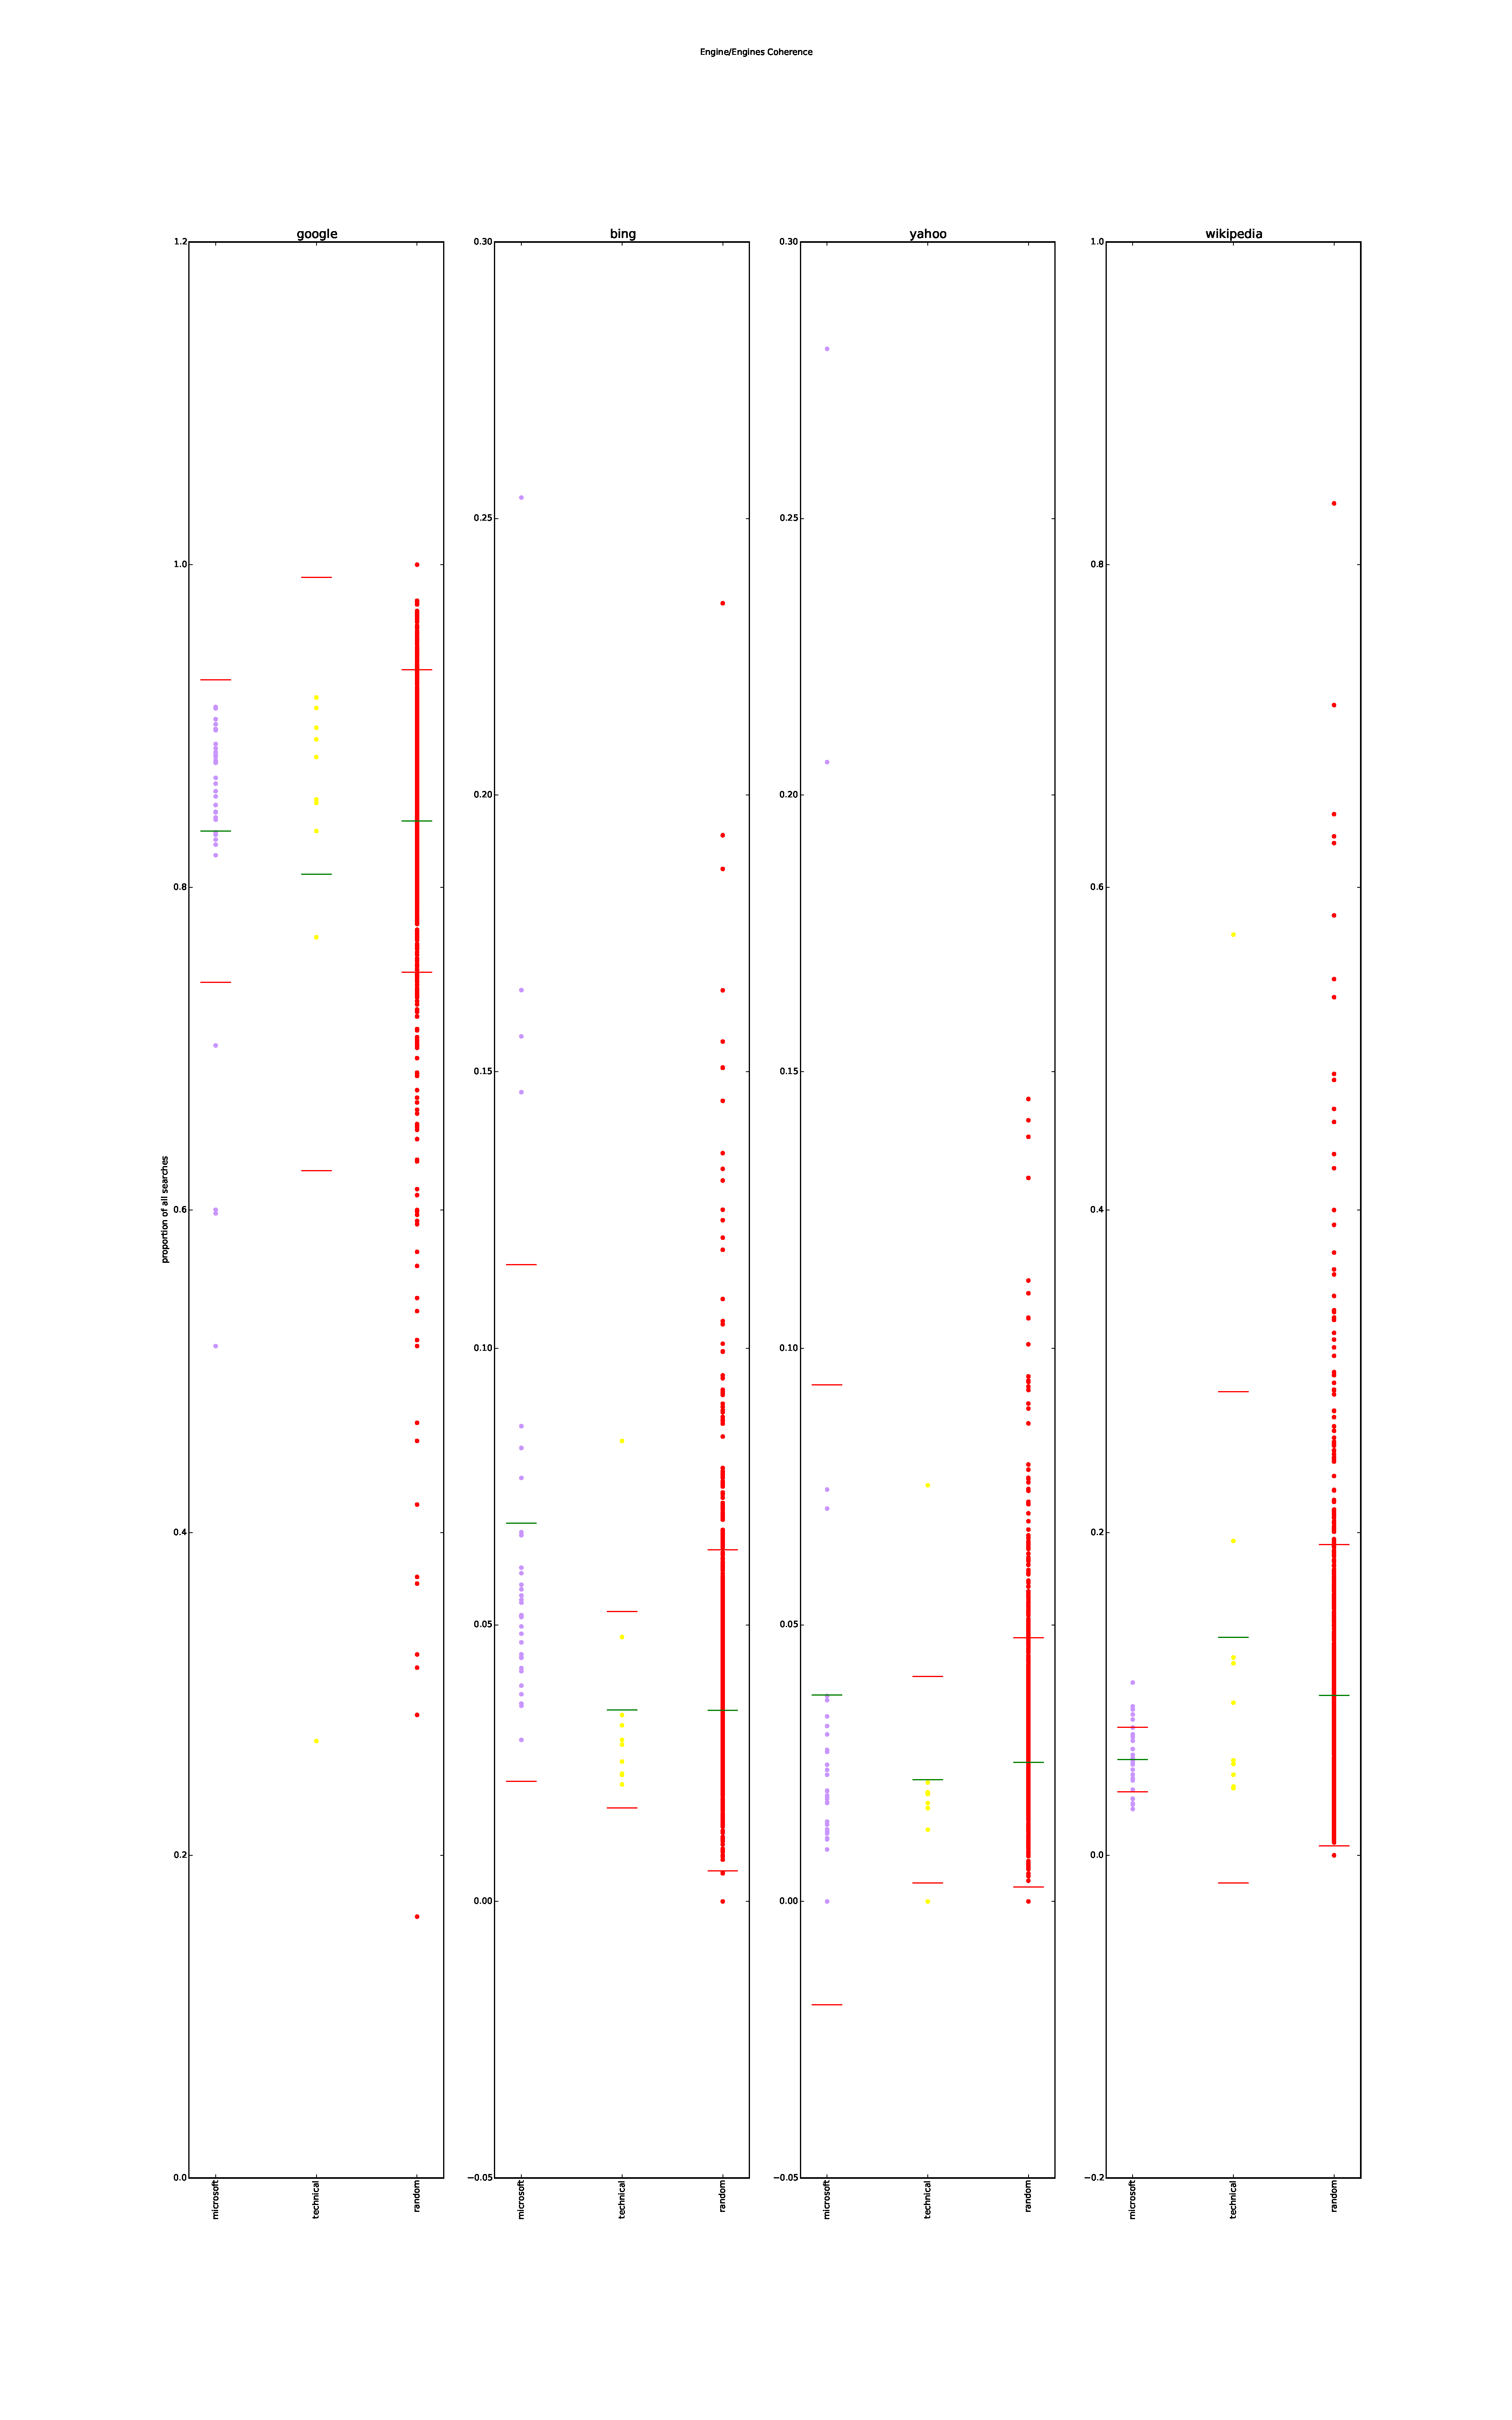
\includegraphics[width=\textwidth]{results/Microsoft_Bing_Engine_Engines_Coherence.pdf}
    \caption{Categories on x axis. Proportions of net engine traffic on y axis. Green line is mean.} \label{fig:ms}
\end{figure}

I also grouped the categories ‘danger’, ‘sexual’, and ‘political’ together as experimental groups, and used scientific jargon as a control group. The idea is that a greater proportion of things that viscerally affect people might be clicked on more often than searched for. The ‘danger’ category does not yet have many samples, so its results aren’t significant. It turns out that political things are actually searched for more commonly than clicked on, compared to random pages. It turns out that sexual things are more commonly clicked on than searched for, compared to random pages. Both of these results are visible in \cref{fig:clickbait}. 

\begin{figure}
    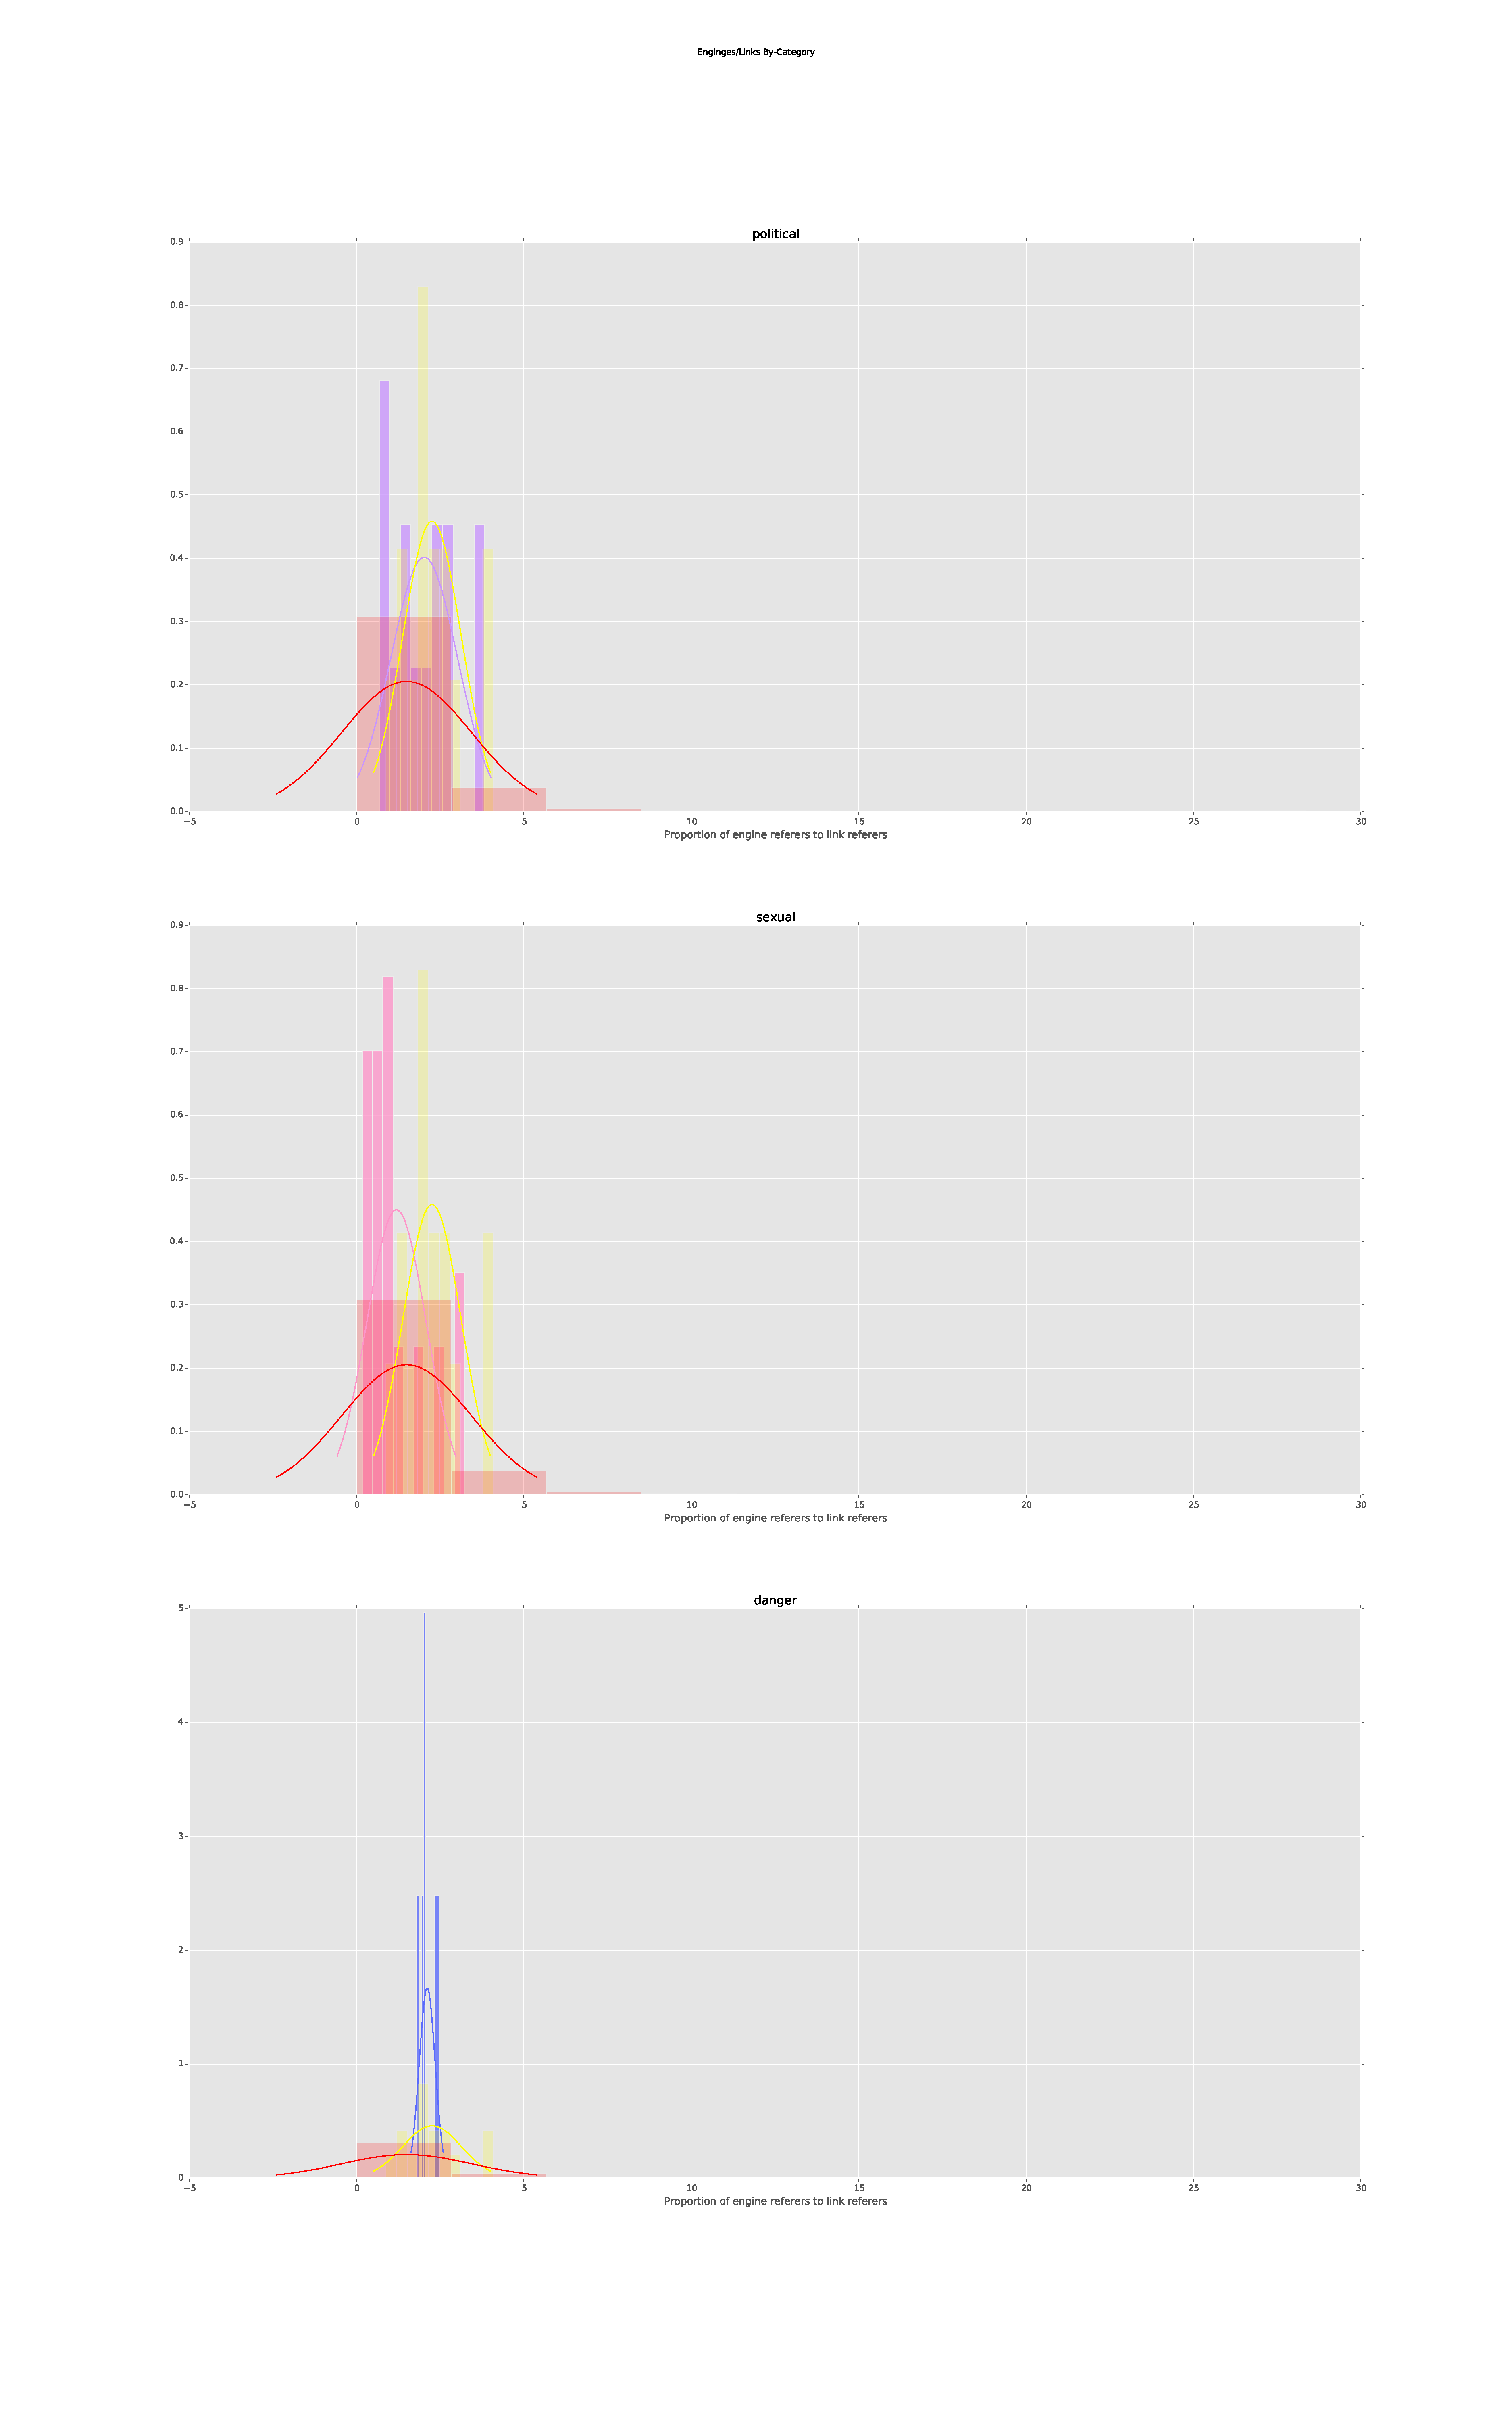
\includegraphics[width=\textwidth]{results/Clickbait_Engines_Links_By-Category.pdf}
    \caption{Y axis is normalized differently according to sample size of category to compare histograms} \label{fig:clickbait}
\end{figure}


I have also posed a few questions that I have not yet answered. Pages which have relatively few total views may have differences in the proportion of people finding them via links versus search engines. People use search engines to learn about things they don’t know much about, so I expect a greater proportion of traffic to obscure pages to come from search engines. Finding the results to this question might have a significance for previous questions. If more commonly visited pages have something characteristic about them, the samples that I manually choose for any question might be biased towards those characteristics when compared to a random sample that also looks at lesser-viewed pages. Although I don’t have any hypothesis, there may be a relationship between the type of noun (person, event, concept, etc) and the proportion of search engine traffic to link traffic. People may search for things they are curious about and then click on the people who are associated with those things. I’m not sure, but it is easy to pose the question.
\end{document}
